%%
%% static_code_analysis_in_ci.tex
%% V0.1
%% 2015/01/22
%% by 
%% Sebastian Funke
%% Hamza Zulfiqar
%% Brian Pfretzschner
%% See:
%% https://github.com/hzulfiqar/SecSoftDev
%% for current contact information.
%%


\documentclass[conference]{IEEEtran}


% *** PACKAGES ***
%\usepackage{algorithmic}
%\usepackage{array}
%\usepackage{mdwmath}
%\usepackage{mdwtab}
%\usepackage{eqparbox}
%\usepackage{fixltx2e}
%\usepackage{stfloats}
\usepackage{cite}       % http://www.ctan.org/tex-archive/macros/latex/contrib/supported/cite/
\ifx\pdfoutput\undefined
\usepackage{graphicx}   % http://www.ctan.org/tex-archive/macros/latex/required/graphics/
\else
\usepackage[pdftex]{graphicx}
\fi
\usepackage{subfigure}  % http://www.ctan.org/tex-archive/macros/latex/contrib/supported/subfigure/
\usepackage{url}        % http://www.ctan.org/tex-archive/macros/latex/contrib/other/misc/
\usepackage[cmex10]{amsmath}    % http://www.ctan.org/tex-archive/macros/latex/required/amslatex/math/
%\usepackage{amsfonts}
\interdisplaylinepenalty=2500
\ifx\pdfoutput\undefined
\usepackage[hypertex]{hyperref}
\else                   % http://www.ctan.org/tex-archive/macros/latex/contrib/supported/hyperref/
\usepackage[pdftex,hypertexnames=false]{hyperref}
\fi



% correct bad hyphenation here
\hyphenation{op-tical net-works semi-conduc-tor}


\begin{document}
%
% paper title
\title{Integration of Static Security Code Analysis\\in Continuous Integration Lifecycles}



%\author{\IEEEauthorblockN{Sebastian Funke}
%\IEEEauthorblockA{Secure Software Engineering\\
%TU Darmstadt\\
%sebastian.funke@stud.tu-darmstadt.de}
%\and
%\IEEEauthorblockN{Brian Pfretzschner}
%\IEEEauthorblockA{Secure Software Engineering\\
%TU Darmstadt\\
%brian.pfretzschner@stud.tu-darmstadt.de}
%\and
%\IEEEauthorblockN{Hamza Zulfiqar}
%\IEEEauthorblockA{Secure Software Engineering\\
%TU Darmstadt\\
%hamza.zulfiqar@stud.tu-darmstadt.de}}



\author{\authorblockA{Sebastian Funke, Brian Pfretzschner, Hamza Zulfiqar}
	\authorblockA{Center for Advanced Security Research Darmstadt\\
		Department of Computer Science\\
		Technische Universit\"at Darmstadt, Germany}}




% use for special paper notices
%\IEEEspecialpapernotice{(Invited Paper)}




% make the title area
\maketitle


\begin{abstract}
\boldmath
In our paper we present our research results for the question: How to integrate static code analysis for security in a common continuous integration (CI) process of software development.
And evaluate the vulnerability reporting capabilities in Jenkins and the open source quality management tool SonarQube.
We used the popular CI tool Jenkins on a NIST standardized C test project\footnote{\url{http://samate.nist.gov/SRD/testsuite.php}} with a variety of vulnerabilities.
Thereby we included a couple of static analysis tools in Jenkins for finding bugs and vulnerabilities during build and after the build process.
Furthermore we analyzed how input validation is deployed in popular PHP frameworks.
\end{abstract}

% no keywords




% For peerreview papers, this IEEEtran command inserts a page break and
% creates the second title. It will be ignored for other modes.
\IEEEpeerreviewmaketitle



\section{Introduction}
% no \IEEEPARstart
Content from our slides...about input validation and how static code analysis works.
Limitation on open source, static analysis tools. Jenkins, SonarQube...and why\cite{IEEEexample:bluebookarticle}.
Content of our paper, what comes when blabla...


\section{Input validation in popular frameworks}
\label{sec:input_validation}
Check those \url{http://codegeekz.com/20-best-php-frameworks-developers-august-2014/} and make a table how input validation is handled there...


\section{Static code analysis in Jenkins}
\label{sec:static_code_analysis_jenkins}
Used test suite: wireshark 1.8 from NIST testsuites with 85 vulnerabilities.
Because its C, because its one of the most security critical languages and there are many good analyzers for C.
Why not Juliet TestSuite with 65 000 vulnerabilities?
Because they are collections of testcases and not a easily build-able project and the analysis and build process would take to long to evaluate the reporting features of the analyzers.


Todo: Table with tools with pros and cons

\begin{figure}[!t]
	\centering
	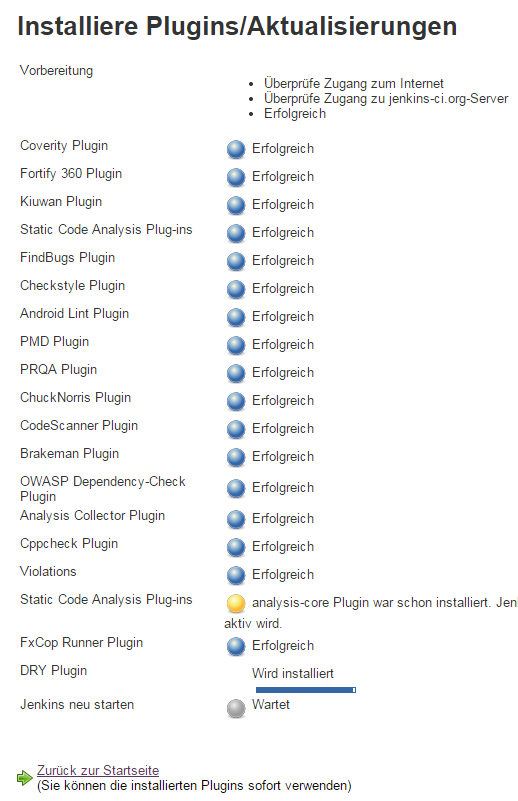
\includegraphics[width=1\linewidth]{img/jenkins-code-analysis-plugins.png}
	\caption{Just a few used Jenkins plugins for static code analysis}
	\label{fig:jenkins-plugins}
\end{figure}


\section{Static code analysis in SonarQube}
\label{sec:static_code_analysis_sonarqube}



\section{Evaluation of reporting capabilities}
\label{sec:evaluation}
Definition for userfriendly vulnerability reporting needed!
Metrics for evaluation of reports needed and need to be mapped on the useabillity definition. 

\subsection{Jenkins}
\label{sec:evaluation_jenkins}

\subsection{SonarQube}
\label{sec:evaluation_sonarqube}




\section{Conclusion}
\label{sec:conclusion}
\begin{itemize}
	\item Conclusion about how input validation is done in frameworks, what can be better ...
	\item Conclusion, is it better to integrate static analysis in Jenkins or just use SonarQube
	....its really not that easy to find the right static code analyzer for your project with a specific programming language. There are lots of open source tools, but very old and just supported by Jenkins over hacks.
	\item Conclusion, is reporting in Jenkins useable
	\item Future work: Using many tools is basically a good idea, because more tools find potentially more vulnerabilities. A future approach would be to implement a tool that can filter all the generated reports. Thereby duplicate vulnerabilities findings can be merged and false positives can be reduced.
\end{itemize}






\section{Sources and useful links}
\begin{itemize}
	\item \href{http://www.crosstalkonline.org/storage/issue-archives/2010/201003/201003-Stiehm.pdf}{Building Security In Using Continuous Integration}
	\item \href{http://www.jetbrains.com/teamcity}{TeamCity}\\
	Supports static code analysis. Also, it can import analysis reports produced by these tools: PMD, PMD/CPD, FindBugs, Checkstyle or JSLint.
	\item \href{http://jenkins-ci.org}{Jenkins}
	\item \href{http://continuum.apache.org}{Apache Continuum}	
\end{itemize}




\bibliographystyle{IEEEtran}
% argument is your BibTeX string definitions and bibliography database(s)
\bibliography{./references}


\end{document}


